\section{Introduction}
\label{sec:introduction}

% state the learning objective 

\hspace{0,5cm} This report is being made for the subject of Circuit Theory and Electronics Fundamentals and is related to the fourth laboratory being its objective to develop an audio amplifier circuit (made of Bipolar Junction Transistors) by choosing the architecture ot the Gain and Output amplifier stages. The circuit is shown in figure \ref{fig:circuito}.
\par In Section~\ref{sec:analysis} a theoretical analysis will be made and it can be decomposed in two stages: the gain stage where the objective is to have the maximum gain possible and the output stage whose objective is to lower the impedance of the amplifier. Secondly, in Section~\ref{sec:simulation} it will be simulated the circuit using ngspice tools. Following with both results from Section~\ref{sec:analysis} and Section~\ref{sec:simulation} being compared and commented in Section ~\ref{sec:comparison}. 
\par Also, it is important to notice that were used two types of BJTs transistors: BC557A (PNP type) and BC547A (NPN type).
\par Finally, the conclusions of this study are outlined in Section~\ref{sec:conclusion}.

\begin{figure}[H] \centering
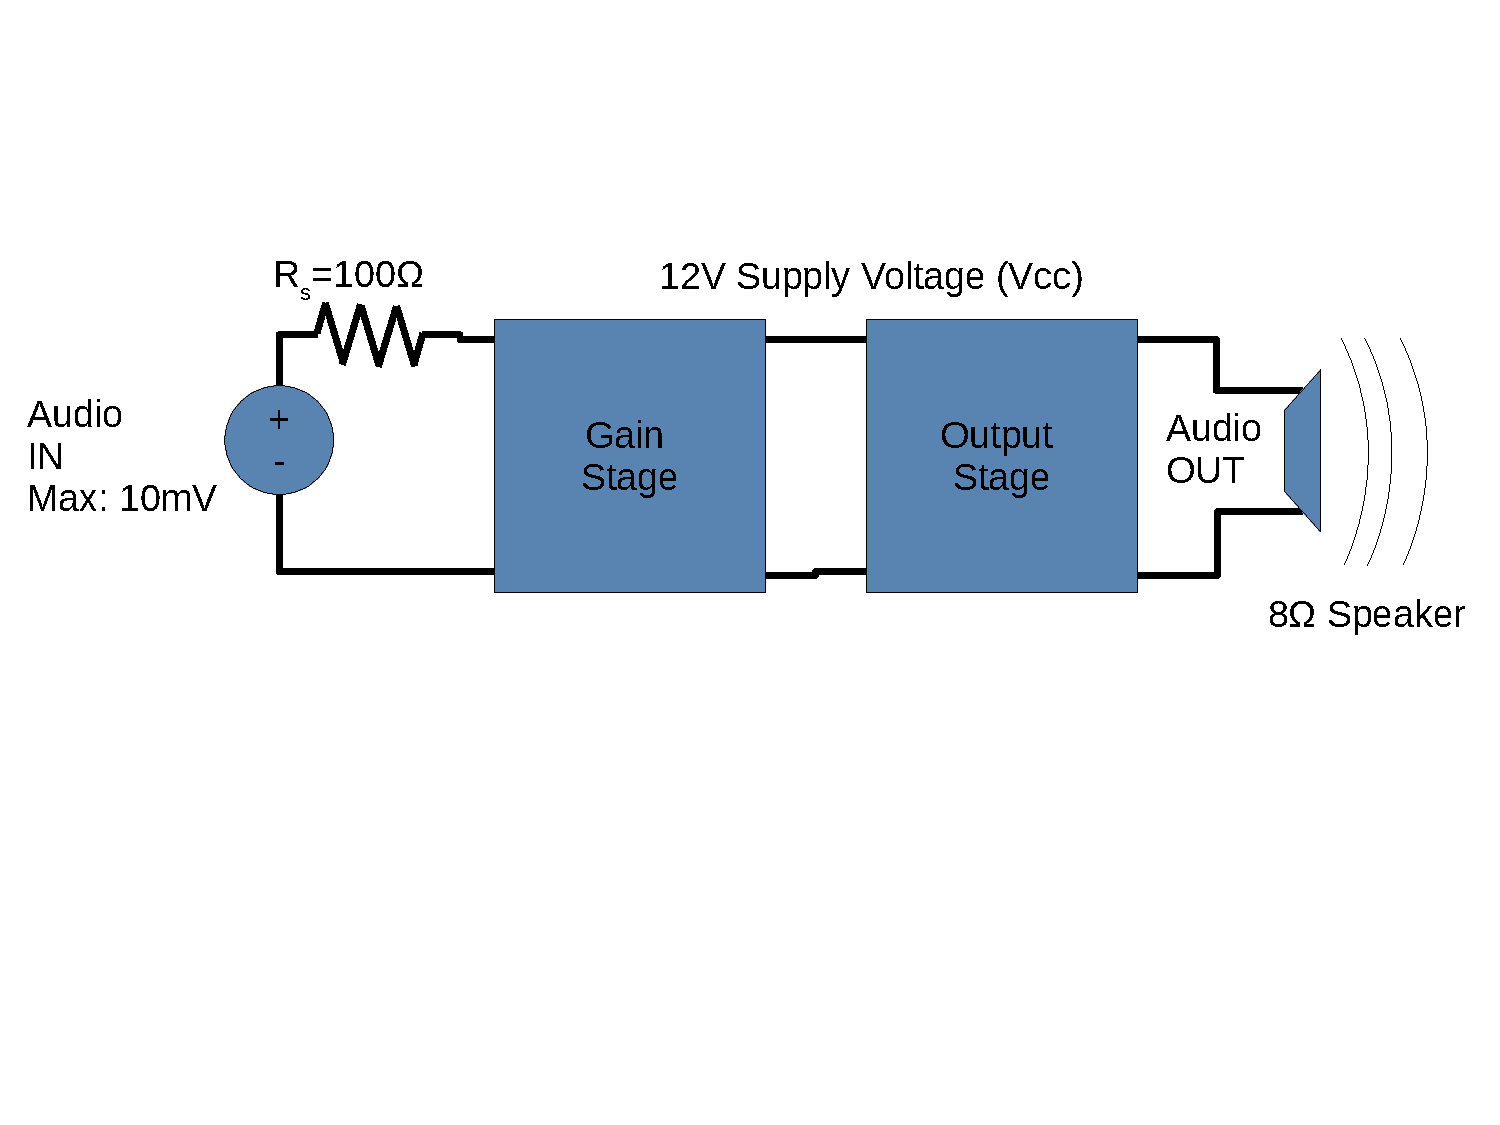
\includegraphics[width=1\linewidth]{circuito.pdf}
\caption{Audio Amplifier Circuit}
\label{fig:circuito}
\end{figure}


